\chapter{Core Language Syntax and Types}\label{chp:qub-language}
In this chapter we give the formal description of \qub{}'s syntax and types. We explain what
it means for a type assignment to exist as binary trees. We then show how we generalize the tree
into a sharing graph and represent it as a collection of three tuple sets in order to simplify our type inference algorithm.

\begin{figure}[h]
  \begin{framed}
    \begin{minipage}{0.35\linewidth}
    \begin{flalign*}
      t, u           &\in \text{Type Variables}\\
      P, Q            &\in \text{Finite Predicate Set}\\
    \end{flalign*}
  \end{minipage}
  \begin{minipage}{0.65\linewidth}
    \begin{flalign*}
      \text{Types}\ \ \  \tau, \upsilon, \phi         &::= t \mid \iota \mid \tau \rightarrow \tau\\
                   &\text{where}\qquad \rightarrow \in \{\tightoverset{\scalebox{0.5}{!}}{\sepimp}, \sepimp, \tightoverset{\scalebox{0.5}{!}}{\shimp}, \shimp \}\\
      \text{Predicates}\ \ \        \pi,\omega        &::= \texttt{Un}\ \tau \mid \texttt{SeFun}\ \tau \mid \texttt{ShFun}\ \tau \mid \tau \geq \tau' \\
      \text{Qualified Types}\ \ \     \rho            &::= \tau \mid \pi => \rho \\
      \text{Type schemes}\ \ \        \sigma          &::= \rho \mid \forall t. \sigma
    \end{flalign*}
  \end{minipage}
  \end{framed}
  \caption{Types \qub{}}
  \label{fig:qub-types}
\end{figure}
% Describe types
The type language consists of type variables ($t$, $u$), built-in types such as integers, booleans ($\iota$), and four function types the
sharing arrow ($\shimp$) and the separating arrow ($\sepimp$) and unrestricted
version of both the function types ($\tightoverset{\scalebox{0.5}{!}}{\shimp}, \tightoverset{\scalebox{0.5}{!}}{\sepimp}$ respectively).
The sharing arrow would mean that the function shares resources with its argument and the separating
arrow would mean that the function does not share resources with its arguments.

% Describe Predicates
The predicate system enhances the expressivity of the type system. Following the same route taken
in Quill \citep{morris_best_2016} we use the predicate $\Un{\tau}$ to denote
that the type $\tau$ is unrestricted. Unrestricted types do not have any resources or whose resources can
be duplicated or deleted easily. Built-in types such as \HaskellF{Int}, \HaskellF{Char} are considered unrestricted types.
We write $\ShFun{\phi}$ to describe that type $\phi$ shares resources with its
argument types and  $\SeFun{\phi}$ to describe that type $\phi$ does not share any resources from its argument types.
Notice that function types can also be unrestricted i.e. they may not have any resources. If a type $\tau$ is unrestricted i.e. it qualifies with predicate
\texttt{Un} and it also qualifies one of the function predicates---\texttt{SeFun} or \texttt{ShFun}---we write
them as $\tightoverset{\scalebox{0.5}{!}}{\sepimp}$ and $\tightoverset{\scalebox{0.5}{!}}{\shimp}$ respectively.
We also define an ordering on types by using the predicate $\geq$. The predicate $\tau \geq \tau'$ holds if the type $\tau'$
is less restricting than $\tau$ or to say $\tau$ has admits more structural rules than $\tau'$ as explained in \cref{sec:quill}.
The predicate entailment relations $P \Rightarrow Q$ are given in \cref{fig:entailment-rules}.

To keep the current system simple we have not included kinds. They are added into this system as a language extension
to enable users to define custom types using type constructors. We describe this extension in \cref{chp:datatypes}.

\begin{figure}[h]\centering
  \begin{framed}
    \begin{minipage}{0.20\linewidth}
      \begin{prooftree}
        \AxiomC{$\pi \in P$}
        \UnaryInfC{$P \Rightarrow \pi$}
      \end{prooftree}
    \end{minipage}%
    \begin{minipage}{0.20\linewidth}
      \begin{prooftree}
        \AxiomC{$\bigwedge_{\pi \in Q} P \Rightarrow \pi$}
        \UnaryInfC{$P \Rightarrow Q$}
      \end{prooftree}
    \end{minipage}%
    \begin{minipage}{0.24\linewidth}
      \begin{prooftree}
        \AxiomC{${\color{white}\bigwedge_{\pi \in Q}}$}
        \UnaryInfC{$P \Rightarrow \Un{(\tau \tightoverset{\scalebox{0.5}{!}}{\sepimp} \tau')}$}
      \end{prooftree}
    \end{minipage}
    \begin{minipage}{0.24\linewidth}
      \begin{prooftree}
        \AxiomC{${\color{white}\bigwedge_{\pi \in Q}}$}
        \UnaryInfC{$P \Rightarrow \Un{(\tau \tightoverset{\scalebox{0.5}{!}}{\shimp} \tau')}$}
      \end{prooftree}
    \end{minipage}

    \begin{minipage}{0.24\linewidth}
      \begin{prooftree}
        \AxiomC{${\color{white}P \Rightarrow \tau \geq \phi t}$}
        \UnaryInfC{$P \Rightarrow \tau \geq (\upsilon \sepimp \upsilon')$}
      \end{prooftree}
    \end{minipage}%
    \begin{minipage}{0.24\linewidth}
      \begin{prooftree}
        \AxiomC{${\color{white}P \Rightarrow \tau \geq \phi t}$}
        \UnaryInfC{$P \Rightarrow \tau \geq (\upsilon \shimp \upsilon')$}
      \end{prooftree}
    \end{minipage}%
    \begin{minipage}{0.24\linewidth}
      \begin{prooftree}
        \AxiomC{$P \Rightarrow \Un{\tau}$}
        \UnaryInfC{$P \Rightarrow \tau \geq (\upsilon \tightoverset{\scalebox{0.5}{!}}{\sepimp} \upsilon')$}
      \end{prooftree}
    \end{minipage}%
    \begin{minipage}{0.24\linewidth}
      \begin{prooftree}
        \AxiomC{$P \Rightarrow \Un{\tau}$}
        \UnaryInfC{$P \Rightarrow \tau \geq (\upsilon \tightoverset{\scalebox{0.5}{!}}{\shimp} \upsilon')$}
      \end{prooftree}
    \end{minipage}

    \begin{minipage}{0.20\linewidth}
      \begin{prooftree}
        \AxiomC{$\tau = \sepimp \vee \tau = \tightoverset{\scalebox{0.5}{!}}{\sepimp}$}
        \UnaryInfC{$P \Rightarrow \SeFun{\tau}$}
      \end{prooftree}
    \end{minipage}%
    \begin{minipage}{0.20\linewidth}
      \begin{prooftree}
        \AxiomC{$\tau = \shimp \vee \tau = \tightoverset{\scalebox{0.5}{!}}{\shimp}$}
        \UnaryInfC{$P \Rightarrow \ShFun{\tau}$}
      \end{prooftree}
    \end{minipage}%
    \begin{minipage}{0.30\linewidth}
      \begin{prooftree}
        \AxiomC{$P \Rightarrow \tau \geq \phi t$}
        \AxiomC{$t\ \text{fresh}$}
        \BinaryInfC{$P \Rightarrow \tau \geq \phi$}
      \end{prooftree}
    \end{minipage}
  \end{framed}
  \caption{Entailment Rules}
  \label{fig:entailment-rules}
\end{figure}

% Describe Typing environment
In normal type systems, the contexts are represented as sets or lists. In logic of \BI{} they are represented as binary trees and are called bunches.
The leaf nodes contain the pair of term and its associated type. Internal nodes of the context tree are
connectives which can either be a semicolon ($;$) or a comma ($,$).
If a bunch $\Delta$ is a subtree of $\Gamma$, the relation is denoted by $\Gamma(\Delta)$.
The bunches have a restriction that no identifier appears more than once. Certain structural rules are restricted on the context
depending on the connectives used. If contexts are combined using a comma ($,$), contraction and weakening is not admissible,
but if the contexts are combined using a semicolon ($;$), it may undergo contraction and weakening. Exchange rule is admissible
in both the connectives. This distinction enables a special treatment for resources in within the language.
By adding resources with a comma constructor in the typing envrionment, the type system will not dispose them off by using the contraction rule,
while non-resourceful objects (or normal propositions) can be added using the semi-colon constructor.
An example bunch is shown in \cref{fig:bunches-bi}. a and b are in sharing while, c is separate from the a and b.
If $\Gamma$ represents the complete context of \cref{fig:bunches-bi}, $\Delta \equiv (a:A; b:B)$ and $\Delta' \equiv (c:C)$
then $\Gamma \equiv \Delta,\Delta'$ and $\Gamma(\Delta)$. In general, two bunches are said to be equivalent ($\Gamma \equiv \Delta$)
if they can be transformed into another by re-associativity.

\begin{figure}[h]
  \begin{framed}
  \begin{minipage}[c]{0.45\linewidth}
  \centering
      \tikzset{every tree node/.style={minimum width=2em},
        blank/.style={draw=none},
        edge from parent/.style=
        {draw,edge from parent path={(\tikzparentnode) -- (\tikzchildnode)}},
        level distance=1.5cm}
      \begin{tikzpicture}
        \Tree
        [.,
        [.;
        [.a:A ]
        [.b:B ]
        ]
        [.c:C ]
        ]
      \end{tikzpicture}
    \caption{Bunch in \textbf{\em BI}}
    \label{fig:bunches-bi}
  \end{minipage}\hfill%
  \begin{minipage}[c]{0.45\linewidth}
  \centering
      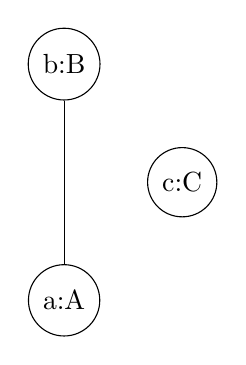
\begin{tikzpicture}
        \node[shape=circle,draw=black] (A) at (0,0) {a:A};
        \node[shape=circle,draw=black] (B) at (0,3) {b:B};
        \node[shape=circle,draw=black] (C) at (1.5,1.5) {c:C};

        \path [-] (A) edge node {} (B);
      \end{tikzpicture}
    \caption{Sharing Graph in \qub{}}
    \label{fig:sharing-graph}
  \end{minipage}
\end{framed}
\end{figure}

In our type system, we generalize the tree approach into a graph where each node represents variables or resources
and the edges between the nodes represent sharing between them. The example in \cref{fig:bunches-bi} can
be represented as what we would call a sharing graph shown in \cref{fig:sharing-graph}. A graph structure, in general,
can represent a binary tree structure and its associated operations. They represent more complex structures than
trees, thus will provide more flexibility in accepting well typed terms in our language making it more expressive.
They also internalize the transformations that are made explicit in the logic of \BI{}. For example, the context tree in \BI{}
$(a:A, a:B), c:C$ is equivalent to $a:A, (b: B, c:C)$ while in \qub{} the sharing graphs of both the trees would be equal.
The sharing graph also preserves the distributive law where $a:A;(b:B,c:D) \vdash (a:A;b:B),(a:A;c:C)$

We define sharing relation, $\Psi$, as a mapping between variables to the collection of variables it is in sharing with.
The relation $\Psi(x, \{y_1, y_2, y_3\})$ holds if $x$ is in sharing with $\{y_1, y_2, y_3\}$.
Domain of $\Psi$ will be defined as $\texttt{dom}(\Psi) = \{x \mid (x, \vec{y}) \in \Psi \}$, where $\vec{y}$
is a shorthand for the denoting collection of variables that are shared with $x$. We can think of $\Psi$ to be similar to $\Gamma$,
but it contains the sharing information instead of the type of the variable. Extending the sharing for a variable will be denoted by $\Psi(x) + y$,
which would mean the variable $y$ is in sharing with $x$. We axiomatize the sharing operation to be reflexive,
symmetric and non-transitive. The sharing relation is non-transitive due to the natural notion of sharing. For example, given three variables,
$x$, $y$, $z$: If $x$ is in sharing with $y$ and $y$ is in sharing with $z$ need not imply $x$ is in sharing with $z$.
So to say,
\begin{flalign*}
 &\forall_{x \in \texttt{dom}(\Psi)}\ x \in \Psi(x) \tag{reflexive}\\
 &\forall_{x,y \in \texttt{dom}(\Psi)}\ \text{if}\ y \in \Psi(x)\ \text{then}\ x \in \Psi(y) \tag{symmetric}\\
 &\forall_{x,y,z \in \texttt{dom}(\Psi)}\ \text{if}\ y \in \Psi(x)\ \text{and}\ z \in \Psi(y)\ \nRightarrow z \in \Psi(x) \tag{non-transitive}
\end{flalign*}

Our final goal is to design a simple type inferencing algorithm for a term language.
Using sharing graphs in implementing typing judgments would make the process considerably complex.
We simplify the sharing graph by flattening it into an adjacency list or a collection of 3 tuple containing the
variable identifier, its type and a collection of variables it shares with. Manipulating lists is much
easier than manipulating graphs. For example, if a resource $x$ has type $\tau$ and it shares with variables $\{y_1, y_2, y_3\}$
we would represent it as $x^{\{y_1, y_2, y_3\}}:\tau$ or just $x^{\bar{y}}:\tau$ for short.
We would write $\Gamma, x^{\vec{y}}:\tau$ to mean $\Gamma \sqcup \{x^{\vec{y}}:\tau\}$.
We can now formally define the typing context or environment for our system as shown in \cref{fig:typing-context}.
\begin{figure}[h]
  \begin{framed}
    \begin{flalign*}
      \text{Typing Context}\ \ \      \Gamma,\Delta     &::= \epsilon \mid \Gamma, x^{\vec{y}}:\sigma
  \end{flalign*}
\end{framed}
  \caption{Typing Context}
  \label{fig:typing-context}
\end{figure}

We define a few auxiliary functions on the
type assignments. \texttt{Vars}($\Gamma$) is the set of all the term variables in $\Gamma$. \texttt{Shared}($\Gamma$) computes
the set of all the term variables that are in sharing with each other. \texttt{Used}($\Gamma$) computes the
union of all the term variables in the type assignment and the term variables shared by each of those.
We define two partial operators on type assignments as shown in \cref{fig:type-assignment-operations}.
The mapping function ($\Gamma^{[\vec{a} \mapsto \vec{b}]}$) extends the sharing relation between the terms. With respect to sharing graphs
it would mean adding edges between the nodes.
\begin{figure}[h]
  \begin{framed}
    \noindent
    \begin{minipage}[h]{0.45\linewidth}
    \begin{flalign*}
      \texttt{Vars}(\Gamma, x^{\vec{y}}:\tau) &= \texttt{Vars}(\Gamma) \cup \{ x \}\\
      \texttt{Shared}(\Gamma, x^{\vec{y}}:\tau) &= \texttt{Shared}(\Gamma) \cup \{ \vec{y} \}\\
      \texttt{Used}(\Gamma) &= \texttt{Vars}(\Gamma) \cup \texttt{Shared}(\Gamma)\\
    \end{flalign*}
  \end{minipage}%
  \begin{minipage}[h]{0.45\linewidth}
    \begin{flalign*}
      (\Gamma, x^{\vec{y}}:\tau)^{[a \mapsto \vec{b}]} &= \begin{cases}
        a \notin \vec{y}\ \ \ \ (\Gamma^{[a \mapsto \vec{b}]}, x^{\vec{y}}:\tau)\\
        a \in \vec{y}\ \ \ \  (\Gamma^{[a \mapsto \vec{b}]}, x^{(\vec{y}\backslash a)\cup\vec{b}}:\tau)
      \end{cases}\\
      \Gamma^{[\vec{a} \mapsto \vec{b}]} &= (\dots((\Gamma^{[a_1 \mapsto \vec{b}]})^{[a_2 \mapsto \vec{b}]})^{\dots})^{[a_n \mapsto \vec{b}]}
    \end{flalign*}
    \end{minipage}
  \end{framed}
  \caption{Auxiliary Functions on Type Assignments}
  \label{fig:multiset-aux-function}
\end{figure}

Two type assignments are said to be in disjoint union ($\circledast$)
if none of the terms used in the type assignments are common with shared terms of other type assignment.
If the type assignments have an exact overlapping of terms being used,
it is said to be in a sharing union ($\varoplus$). The ($\#$) in ($\circledast$) represents disjoint check and we use
the standard notion of set equality for checking sharing union.

\begin{figure}[h]
  \begin{framed}
    \begin{flalign*}
      \Gamma \circledast \Gamma' &= \Gamma \sqcup \Gamma' \qquad
           \texttt{if}\ \texttt{Vars}(\Gamma) \mathbin{\#} \texttt{Used}(\Gamma') \wedge \texttt{Vars}(\Gamma') \mathbin{\#} \texttt{Used}(\Gamma)\\
      \Gamma \varoplus \Gamma'   &= \Gamma \sqcup \Gamma' \qquad
           \texttt{if}\ \texttt{Used}(\Gamma) = \texttt{Used}(\Gamma')
    \end{flalign*}
  \end{framed}
  \caption{Type Assignment Operations}
  \label{fig:type-assignment-operations}
\end{figure}


\begin{figure}[h]
  \begin{framed}
    \begin{flalign*}
      \text{Term Variables}\ \ \  x, y, z  &\in \text{Var} \nonumber\\
      \text{Expressions}\ \ \     M, N     &::= x \mid \lambda^{\sepimp}x. M \mid \lambda^{\shimp}x. M \mid M N \mid \Let{x}{M}{N}\nonumber
    \end{flalign*}
  \end{framed}
  \caption{Term Language}
  \label{fig:qub-terms}
\end{figure}
% Describe the language here

% Describe terms and patterns
Our term language is similar to that of simply typed lambda calculus involving variables and term application
but we have two types of lambda expressions, the sharing lambda ($\lambda^{\shimp}$) denotes sharing
of the argument term with the expression $M$ and the separating lambda term ($\lambda^{\sepimp} $) that implies
the argument term has a separating context with the expression $M$. We also have $\texttt{let}$
construct to enable parametric polymorphism.

We work in a call-by-value semantics similar to Quill\citep{morris_best_2016} and F$^{\circ}$\citep{mazurak_lightweight_2010} as it is possible
that functions may not be evaluated in call-by-name or call-by-need semantics that would break the linearity property.


%%% Local Variables:
%%% mode: latex
%%% TeX-master: "../thesis-ku.tex"
%%% End:
